\documentclass[tikz,border=2pt]{standalone}
\usepackage{amsmath,amssymb}
\usepackage{tikz}
\usetikzlibrary{arrows.meta}

\begin{document}
% Vector addition: add coordinates, i.e. put the arrows tip to tail (parallelogram rule).
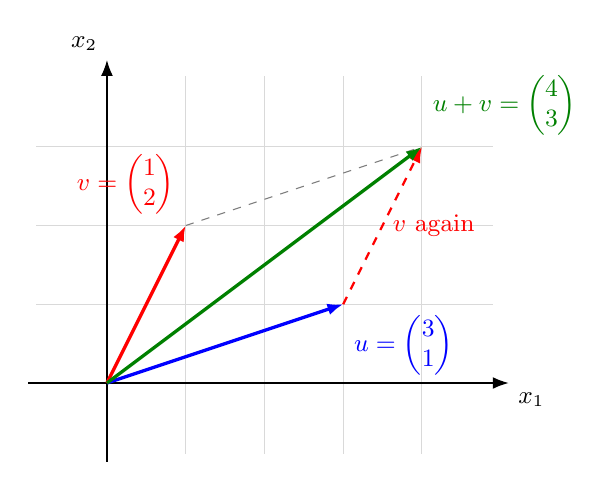
\begin{tikzpicture}[every node/.style={font=\small}, >={Latex[length=2mm]}]
	\draw[gray!30, step=1] (-0.9,-0.9) grid (4.9,3.9);
	\draw[->] (-1,0) -- (5.1,0) node[below right] {$x_1$};
	\draw[->] (0,-1) -- (0,4.1) node[above left] {$x_2$};
	\draw[->, blue, very thick] (0,0) -- (3,1) node[below right] {$u=\begin{pmatrix}3\\1\end{pmatrix}$};
	\draw[->, red, very thick] (0,0) -- (1,2) node[above left] {$v=\begin{pmatrix}1\\2\end{pmatrix}$};
	\draw[->, red, thick, dashed] (3,1) -- (4,3) node[midway, right] {$v$ again};
	\draw[dashed, gray] (1,2) -- (4,3);
	\draw[->, green!50!black, very thick] (0,0) -- (4,3) node[above right] {$u+v=\begin{pmatrix}4\\3\end{pmatrix}$};
\end{tikzpicture}
\end{document}
